\documentclass[aps,prl,reprint,floatfix,superscriptaddress]{revtex4-1} %might want some options later
\usepackage{graphicx}
\usepackage{amsmath}
\usepackage{float}
\usepackage{hyperref}


\begin{document}

\floatstyle{ruled}
\newfloat{program}{ht}{lop}
\floatname{program}{Example }

\title{Quantum Circuit Viewer}
\date{\today}
\author{Alex \surname{Parent}}
\email{aparent@uwaterloo.ca}
\author{Jacob \surname{Parker}}
\email{j3parker@uwaterloo.ca}
\affiliation{Institute for Quantum Computing, University of Waterloo, Waterloo, ON, Canada}
\author{Dmitri \surname{Maslov}}
\email{dmaslov@iqc.ca}
\affiliation{Institute for Quantum Computing, University of Waterloo, Waterloo, ON, Canada}
\affiliation{National Science Foundation, Arlington, VA, USA}
\begin{abstract}
Quantum Circuit Viewer (QCViewer) is a software tool for the design and simulation of 
quantum circuits.  It allows users to test new circuit designs and make publication 
quality diagrams with an easy to use graphical interface.  Supported features also include
simulation of the circuit while graphically displaying the current state.
\end{abstract}
\maketitle

\section{Introduction}
In creating QCViewer our goal was to develop a convenient tool that would be useful to
the quantum computing community for both research and educational purposes. QCViewer 
provides a drag and drop interface for circuit design.  This makes it easy to quickly
test out new algorithm and circuit design ideas.  In order to make the diagrams useful for presentation 
(e.g., Adobe Illustrator, PowerPoint) and publication (e.g., LaTeX) we provide the ability to export images in scalable
vector graphics (.svg) and portable network graphics (.png).
\section{Circuit Format}
To store circuits we use our own circuit format which was somewhat 
inspired by the ``.tfc'' format used on the ``Reversible Logic Synthesis Benchmarks Page''\cite{maslovBench}, and ``.tfc'' files are valid ``.qc'' files (but not the other way around).
We use ``.qc'' as the extension for our circuit files.
To keep this submission short, we will illustrate the construction of a circuit for Grover's algorithm.  The representation we have chosen is 
taken from \cite{nielsen2000quantum}, page 256. It can be found in the software distribution as \verb+demos/grover.qc+.
\subsection{Header}
\begin{program}
\begin{verbatim}
.v a b c d e Workspace
.i a b c d e Workspace
.o a b c d e
\end{verbatim}
\caption{Header example.}
\label{l:head}
\end{program}
This and follow up sections describe the circuit format. 

The ``.v'' list defines names of the circuit qubits. A qubit name may be any ASCII text composed with letters and numbers. The ``.i'' list specifies which %%@
qubits accept primary inputs.
The ``.o'' list reports primary outputs.
There is also an optional ``.ol'' list which allows to alternate names to be specified for the output labels. Finally, an optional ``.c'' list is used to %%@
specify the values of input constants. See Example \ref{l:head} for a sample header.

\subsection{Main Circuit}
The main circuit is specified between the ``\verb+BEGIN+'' and ``\verb+END+'' tags.  Each line contains a gate name followed by labels
specifying which qubits the gate effects, with the first set of inputs being the controls
and the last set of inputs of proper size being the target(s) of the gate.
An apostrophe after a qubit name indicates that the control is negative. For example, \verb+T a b' c+ specifies a Toffoli gate on
qubit $c$, positive control from qubit $a$ and negative control from qubit $b$. Note that negative controls are drawn with a white circle.
In addition to multiple control Toffoli gates with possible control negations, our software readily supports gates X 
(notation \verb+X+; same as Toffoli, \verb+T+),Y (notation \verb+Y+), Z (notation \verb+Z+), Hadamard (notation \verb+H+), 
SWAP (notation \verb+F+) and their controlled versions. 
Single qubit rotations X, Y, and Z are also supported using the R gate, for example 
\verb+R(X0.2)+ would preform a rotation by $(0.2)\pi$ around the x axis. 

Additional gates may be specified on the same line using semicolons for separation. When generating a diagram for a circuit, 
the gates are packed into columns in a greedy fashion. Empty lines between gates will force a column break.

\subsection{Sub-Circuits}
A subcircuit can be specified between the ``\verb+BEGIN <circuit name> (<arg> ...)+'' and ``\verb+END <circuit name>+'' tags. The arguments to a subcircuit are the names of the input qubits. The scope of these arguments is exclusive to the subcircuit, and a subcircuit may not use the global qubit names (it is valid, however, for an argument to a subcircuit to have the same name as a global qubit name). A subcircuit can then be included
in the main circuit as if it were a gate. The qubits it is applied to are mapped to the arguments of the subcircuit. We now build the complete ``.qc'' for Grover's algorithm 
using subcircuits and loops that are introduced in the next section (the header is taken from Example \ref{l:head}). Figure \ref{f:grover} is the diagram that QCViewer generates for the file content shown in Example \ref{l:circuit}.  The usefulness of subcircuits and loops is demonstrated in the
unrolled version of the circuit for Grover's algorithm in Example \ref{l:netlist} and its circuit diagram in Figure \ref{f:netlist}.
\begin{program}

\begin{verbatim}
.v a b c d e Workspace
.i a b c d e Workspace
.o a b c d e

BEGIN 5H (a, b, c, d, e)
H a; H b; H c; H d; H e
END 5H

BEGIN GroverIterate (a, b, c, d, e, Workspace)
H Workspace
T a' b' c d e' Workspace
H Workspace
5H a b c d e
X e
Z a' b' c' d' e
X e
5H a b c d e
END GroverIterate

BEGIN
H5 a b c d e
GroverIterate^4 a b c d e Workspace
END
\end{verbatim}
\caption{Circuit file for Grover's algorithm.}
\label{l:circuit}
\end{program}
\begin{figure}
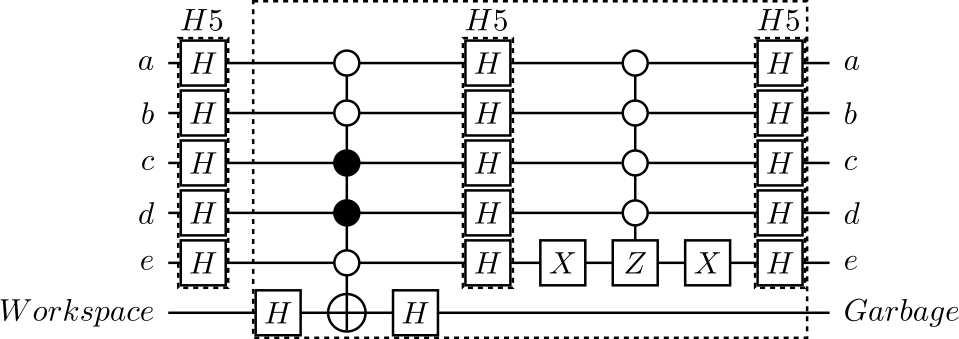
\includegraphics[scale=0.32]{grover_circuit}
\caption{Circuit diagram for Grover's algorithm searching for the item 00110 marked by the Toffoli gate 
``T a' b' c d e' Workspace''. Note that the single iterate, shown in the blue box, is scheduled to be 
executed four times as indicated in blue font above the box.}
\label{f:grover}
\end{figure}

\subsection{Loops}
Loops allow certain parts of the circuit to be executed multiple times. We will use one to perform Grover's iterate repeatedly. They are specified in the file format
using the exponent symbol and subcircuits. For example ``\verb+GroverIterate^4 a b c d e Workspace+'' specifies that the subcircuit ``\verb+GroverIterate+'' %%@
should be run four times on the qubits a, b, c, d, e and Workspace.
\subsection{Gates}
Gates are specified in a gate library file to allow custom gate sets to be added easily. For example, the specification of the Hadamard gate
can be found in Example \ref{l:gate}.
\begin{program}
\begin{verbatim}
NAME Hadamard
SYMBOL H
1/sqrt(2) ,  1/sqrt(2)
1/sqrt(2) , -1/sqrt(2)
\end{verbatim}
\caption{Gate library specification of the Hadamard gate.}
\label{l:gate}
\end{program}

\section{Circuit Design}
Circuits may be written directly in the specified file format as an ASCII file, or drawn graphically using drag-and-drop interface.  Gates can be placed %%@
by dragging them directly onto qubit wires.
Controls are then edited by entering control editing mode and clicking on qubit wires (two clicks to place a negative control).

\section{Circuit Simulation}
Our circuit simulator is state-vector based. The results of the simulation of Grover's algorithm are shown in Figure \ref{f:state}. Breakpoints can be inserted into the circuit to pause the simulation at specific points.  The results of the simulation can be displayed as graphs of the either the probability distribution, real amplitudes or imaginary amplitudes of the state in the computational basis.
\subsection{State Entry}
Input state may be specified using Dirac notation with states being automatically normalized if needed. The input to the circuit implementing Grover's algorithm as illustrated in Figure \ref{f:grover} is ``\verb$|0>^5|1>$'' or more simply 
``\verb$|000001>$''. More complex inputs for other circuits are also supported, e.g., ``\verb$(|0>+|1>)^4 + 3/4|1011>$''.
\begin{figure*}[ht]
\includegraphics[scale=0.35]{simulate}
\caption{The first row shows the state $(H|0\rangle)^{\otimes 5}|1\rangle$, and the subsequent rows show the state as it goes through four iterations of the Grover's iterate. The
diagram for the circuit that generated these pictures can be seen in Figure \ref{f:grover}.}

\label{f:state}
\end{figure*}

\section{Software}
The executable for QCViewer can be obtained from the website \url{http://qcirc.iqc.uwaterloo.ca/}.

\begin{program}
\begin{verbatim}
.v a b c d e Workspace
.i a b c d e Workspace
.o a b c d e

BEGIN
H a; H b; H c; H d; H e; H Workspace
T a' b' c d e' Workspace
H a; H b; H c; H d; H e; H Workspace
X e
Z a' b' c' d' e
X e

H a; H b; H c; H d; H e; H Workspace
T a' b' c d e' Workspace
H a; H b; H c; H d; H e; H Workspace
X e
Z a' b' c' d' e
X e

H a; H b; H c; H d; H e; H Workspace
T a' b' c d e' Workspace
H a; H b; H c; H d; H e; H Workspace
X e
Z a' b' c' d' e
X e

H a; H b; H c; H d; H e; H Workspace
T a' b' c d e' Workspace
H a; H b; H c; H d; H e; H Workspace
X e
Z a' b' c' d' e
X e

H a; H b; H c; H d; H e
END
\end{verbatim}
\caption{Complete circuit netlist in ``.qc'' format for Grover's algorithm used as example written without the use of subcircuit and loop features.}
\label{l:netlist}
\end{program}
\begin{figure*}[ht]
\includegraphics[scale=0.3]{grover_netlist}
\caption{Complete/unrolled circuit diagram for Grover's algorithm searching for the item 00110.}
\label{f:netlist}
\end{figure*}

\bibliography{QCV}
\end{document}
